Despite the conceivable advantages of NVRAM, there are also challenges to be
addressed. Although most issues are of practical nature there also are
conceptual concerns.

\paragraph{Unintended Durability}

The key feature of NVRAM is to retain its data across restarts. However, not all
data are necessarily intended to be durable. Notable examples include transient,
confidential, and corrupt data. The former comprises data which may not be valid
after a system restart, as is the case with data related to machine or device
state.

Other data such as passwords, encryption keys, or decrypted data may be
confidential and should not be durable. It has been shown that even volatile RAM
holds its charge long enough so that a module can be moved to an attacker's
machine for read-out \cite{halderman2008lest}. By cooling the module, capacitor
discharge can be slowed so that it can be moved to another machine where its
content may be read and parsed. Despite being countered with hardware
scramblers, researchers still managed to apply variations of the technique and
obtain vital information \cite{yitbarek2017cold}. Such attacks would be trivial
on NVRAM, as durability is its primary feature \cite{bailey2011operating}. Of
course, confidential data could be overwritten with zeros after usage, but there
is always a possibility that a crash might prevent such clean up tasks from
completing. That said, sensitive data should at all times remain in volatile
memory and be nulled after use. Although information security is an important
matter, this thesis does not address such issues. Although it is important,
information security in terms of attack resilience contributes little to the aim
of this thesis and is therefore not addressed further. Also, since volatile RAM continues to be available, there is no need to use NVRAM for sensitive data.

When an operating system or application behaves in erratic fashion or crashes it
may produce corrupt data in memory. Unless memory is cleared or rewritten,
systems incorporating NVRAM could face durable memory corruptions. The latter
may lead to an unstable system producing even more corrupted data. Although the
same is true for conventional non-volatile memory, it is still operated through
the operating system in terms of an API and volatile page caches. NVRAM on the
other hand is expected to be connected to the memory bus, enabling unbuffered
access through virtual memory addresses. This makes NVRAM vulnerable to stray
writes \cite{condit2009better, venkataraman2011consistent}. However, it has been
shown that, compared to disk storage, stray writes do not occur significantly
more often in NVRAM \cite{chen1996rio}. That said, stray writes are not considered an issue in this work.

\paragraph{Memory Management}

NVRAM is a new type of memory that can also be used as durable mass storage. In
order to benefit from this new technology, both platforms and operating systems
need to find ways to efficiently manage it. There are several issues to be
addressed in this area.

% Memory Interface

An important aspect in managing NVRAM is the memory interface. Recent research
suggests that NVRAM will be attached to the system memory bus using the DIMM
format known from DRAM \cite{volos2017whisper, oukid2017data, andrei2017sap,
intel2017nvdimm}. A decisive advantage of this approach is much lower latencies
compared to the alternative IO bus. Another reason is that in a previous effort
to produce NVRAM, known as NVDIMM, modules have also been integrated this way
\cite{dulloor2014system, huang2014design}. Consequently, system designers can
build on an existing software stack. Still, there are drawbacks to be
considered. Clearly, the number of available DIMM slots in a machine is limited,
so NVRAM may not scale well for mass storage. That situation is especially
relevant in hybrid systems containing both RAM and NVRAM. Also, in hybrid
systems both kinds of memory are likely to be attached to the same memory
interface thus sharing its bandwidth.

With NVRAM devices integrated into the system, programmers still need a way to
access it. Several approaches have been proposed to this end
\cite{volos2017whisper}. While it is always possible to operate on NVRAM by
mapping individual device regions into virtual memory, there are considerable
weaknesses to this approach \cite{condit2009better, volos2011mnemosyne,
dulloor2014system, volos2017whisper}. A major challenge of working with NVRAM is
to provide consistency guarantees across possible system failures. Yet, systems
are largely unaware of these circumstances. With raw device access which is
already error-prone, the complex task of preserving consistency is handed to the
programmer. Another challenge is that virtual memory mappings are volatile and
may no longer be valid after a restart.

Therefore, it has been proposed to rely on dedicated high-level programming
primitives as in Mnemosyne, NV-Heaps, and NVML \cite{volos2011mnemosyne,
coburn2011nv_heaps, intel2017nvml}. These systems provide interfaces for memory
allocation and consistent updates based on transactions. An important
distinction to the previous low-level approach is that memory is accessed
through an NVRAM-aware API instead of basic load and store statements. The
difference is that the latter have no knowledge of non-volatile memory and its
implications.

\begin{figure}[!ht]
    \centering
    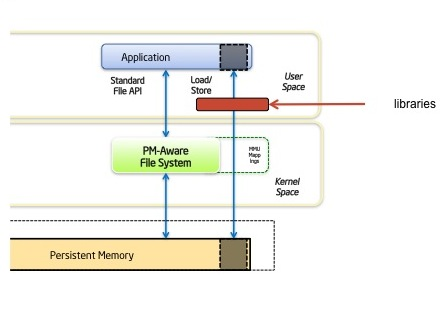
\includegraphics[scale=0.75]{figures/nvml-arch.jpg}
    \caption{System hierarchy indicating the position of NVML in red \cite{intel2014nvml}}
    \label{fig:nvml}
\end{figure}

Another discussed approach to manage NVRAM is through designated file systems
\cite{oukid2017data, andrei2017sap}. File systems provide a well-known and
suitable abstraction for non-volatile storage. In order to enable regular memory
access in a load-store manner, individual files can be mapped into virtual
memory. However, traditional file systems are not directly well-suited for use
with NVRAM. One reason is that most operating systems provide a page cache which
is used by file systems to defer expensive disk IO. In the case of NVRAM, page
caches may be no longer needed, as updates to NVRAM incur far less latency
compared to other non-volatile memories. In this regard, page caches even add
overhead instead of mitigating it. Apart from that, they add a level of
indirection which makes writes to NVRAM more likely to be torn by failures.
Also, traditional file systems are usually designed for block-oriented devices
which may no longer be the best option. Therefore, several NVRAM-aware file
systems have been proposed \cite{condit2009better, wu2011scmfs,
dulloor2014system, xu2016nova}. The key feature of these file systems is a
zero-copy mechanism by circumventing page caches. This enables true store-load
semantics for memory-mapped files. Other aspects include attempts to leverage
the byte-addressable nature of NVRAM and crash-related consistency issues.

Unfortunately, as of this writing there is no evident consensus regarding the
programming model to use for NVRAM \cite{boehm2016persistence}. Still,
middlewares such as NVML appear to be gaining the upper hand
\cite{oukid2017data, volos2017whisper, malinowski2017using, andrei2017sap}.

\paragraph{Consistency}

A notorious problem with NVRAM is consistency in case of crashes
\cite{condit2009better, dulloor2014system, oukid2017data}. Due to the complex
nature of this subject, further discussion is deferred to the next section.
